\section{Modelos}

A continuación detallamos los modelos que han sido diseñados, mostrando el nombre del modelo, un diagrama de clases contenido para cada modelo, y una documentación generada a partir de las propias anotaciones del modelo.

El generador de aplicaciones \gls{iot} cuenta con los siguientes grupos de modelos:

\begin{itemize}
\item Modelos relativos al sistema de eventos.
Todo el sistema depende de estos modelos, eventos y actuadores.

\item Modelos relativos al protocolo de comunicación. Modela las diferentes partes dentro del modelo de comunicación. Eventos, seguridad, estado de salud.

\item Modelos relativos al propio sistema \gls{iot}. Modela la composición básica del sistema, entradas/salidas, archivos, gráficos, sonidos.

\item Modelos relativos al servidor, usuarios, seguridad.
\end{itemize}

Para todos los modelos analizados, mostraremos su diagrama de clases, generado a partir de la transformación creada con \gls{sirius} \cite{sirius} y en algunos de ellos, esquemas en formato \gls{ecore} tree/doc... como anexo para un mayor entendimiento y fácil lectura de esta memoria.

Debido a que el código fuente es muy extenso, no será incluido en la sección anexos y  podrán ser descargado en formato \gls{zip} en la siguiente URL: \textcite{tfm_cesarlaso_codigo}

\subsection{Modelos relativos al dominio del dispositivo IOT}

\subsubsection{Modelo Programa}

Este modelo conforma la base del programa que posteriormente definiremos en el \gls{dsl}. Es la base del proyecto, a partir de este \gls{metamodelo}, generaremos programas mediante un \gls{dsl} creado con \gls{xtext}. 

Este modelo representa un programa \gls{iot} en el que tenemos una serie de entradas, ya sean desde el propio \gls{gpio}, una serie de entradas remotas y acciones tanto en el propio \gls{gpio} como notificaciones remotas.

Como ejemplo, imaginemos un dispositivo \gls{iot} de lo más simple, con una sola entrada digital, utilizado para contabilizar monedas de una máquina de refrescos. Mediante el \gls{dsl} que definimos en este proyecto podríamos generar un programa para una plataforma determinada que cumpla con las siguientes características: Gestión de la interrupción \gls{gpio} asociada a dicho evento de pulso de entrada de moneda, notificación a servidor de este evento,  control de salud del propio dispositivo, etc.

El programa define una serie de \gls{gpio} pin, indicando estos con un alias, es decir, podemos asignar un nombre a una entrada, por ejemplo, \gls{led} rojo \textrightarrow pin1. Cuenta con asignación de nombres de eventos remotos, y rutas de archivos a utilizar por el programa. Un programa cuenta con una serie de estados, necesario indicar el estado principal de arranque de este y posibilitando cambiar de estado. Un ejemplo de uso real es el testeo en el arranque de los diversos indicadores \gls{led} u otras entradas/salidas, y una vez terminado, pasar a un estado de error en caso de fallo, y en caso de funcionamiento normal, pasar al estado del programa principal.


En la figura \ref{fig:modelo_iot_programa_classes} podemos visualizar en formato diagrama de clases \gls{uml} el modelo \textit{Program}.

\begin{figure}
	\centering
    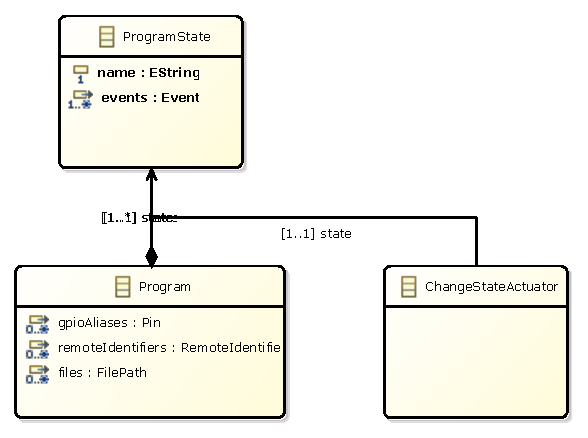
\includegraphics[height=0.3\textheight]{images/models/programs_class_diagram.pdf}
    \captionmodeloclase{Programa IOT}
    \label{fig:modelo_iot_programa_classes}
\end{figure}

\clearpage

\subsubsection{Modelo Operating System Actuators}

Nuestra abstracción de un sistema \gls{iot} necesita contar con una serie de elementos que habitualmente encontramos proporcionados por los sistemas operativos.

Para ello necesitamos modelar estos elementos que utilizaremos desde nuestro \gls{dsl}.

Este modelo, representado en la figura  \ref{fig:modelo_operatingsystemactuators_classes}, representa las funcionalidades básicas que necesitamos por parte del sistema operativo para el funcionamiento de nuestros dispositivos \gls{iot}. Cuenta con una muestra de las tareas que podría implementar nuestro \gls{dsl}, tareas de alto nivel tales como: descarga de archivos, ejecución de programas del sistema, visualización de imágenes en pantalla y reproducción de archivos de audio o vídeo.

\begin{figure}[htp]
	\centering
    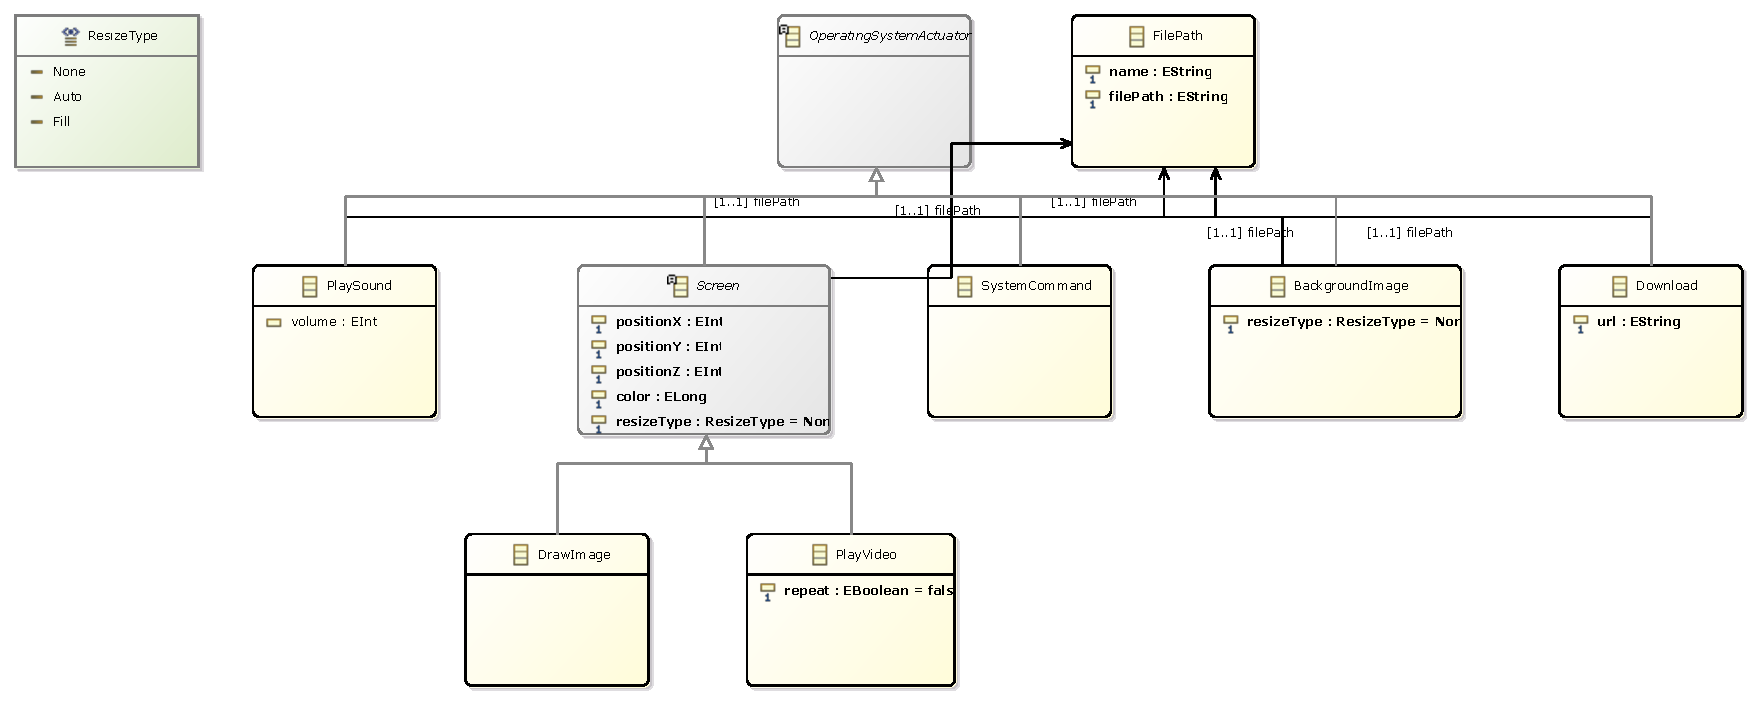
\includegraphics[height=0.3\textheight]{images/models/operatingsystemactuators_class_diagram.pdf}
    \captionmodeloclase{OperatingSystemActuators}
    \label{fig:modelo_operatingsystemactuators_classes}
\end{figure}

\subsubsection{Modelo GPIO}

El modelado de las entradas y salidas en una placa hardware (o emulada) con soporte \gls{gpio} es una de las partes más importante del dispositivo \gls{iot}. Mediante este componente, podremos interactuar con otros dispositivos externos tales como sensores digitales, analógicos, actuadores, etc.

La representación de los modelos, se hará en tres grupos lógicos para su mejor modelado y separación de tareas:  gpio, gpio events y gpio actuators.



En estos modelos definiremos de una forma abstracta estos conceptos para poder interactuar más adelante con ellos.

Los dispositivos \gls{gpio} cuentan con una serie de entradas analógicas o digitales. Muchos de ellos tienen entradas con múltiple funcionalidad pudiendo comportarse como entradas digitales o analógicas vía configuración en tiempo de ejecución. Así mismo, son capaces de funcionar en otras modalidades tales como \gls{rs232} o \gls{i2c}, compartiendo la misma entrega física entre las diversas opciones. Esto quiere decir, que podemos corromper hardware si por error cambiamos un valor de una variable en ejecución, algo que en un lenguaje general debería ser permitido, en nuestro \gls{dsl} no deberíamos dejar, con lo que nuestro programa sería válido en compilación.

Esta funcionalidad tan específica, deberá quedar fuera del modelo, debiéndose soportar en el código no generado automáticamente a partir de los modelos.

Debido a que posteriormente en la sección \gls{dsl} crearemos un lenguaje de tipado fuerte, modelaremos las entradas / salidas especificando el tipo de estas (digital / analógico), evitando posibles fallos en hardware si por ejemplo activamos una salida en un dispositivo de entrada (pudiendo incluso quemar el dispositivo sino incluye algún tipo de resistencia previa).

Otra funcionalidad igualmente importante es la capacidad que tienen estos dispositivos de generar interrupciones vía hardware en el momento de cambio de estado de la señal digital, algo necesario para nuestra definición posterior de sistema de eventos, soportado en mayor medida por este tipo de dispositivos.

En el caso de los sistemas que no posean la característica de interrupción vía hardware, deberá ser emulada mediante software realizando polling sobre el estado de la entrada en cuestión. En el caso de dispositivos con sistema operativo de propósito general como Raspberry PI, se realizará en el hilo principal. En el caso de Arduino, la consulta se realiza dentro del \gls{mainloop}.

Esta casuística de emulación de interrupción vía software no quedará definido en este meta-modelo sino que será definido en la implementación a código final de la plataforma en cuestión.

Nuestro modelo \gls{gpio}, cuenta con una serie de funcionalidades declarativas, permitiendo al desarrollador especificar una serie de tareas sin saber como en capas inferiores las realiza la plataforma. Podemos ver ejemplos como: ButtonInputAccumulator, evento por el cual cada vez que pulsamos un botón (cambiamos de estado durante un tiempo mínimo una entrada \gls{gpio}), lanzamos un evento con un contador de veces.

En la figura \ref{fig:modelo_iot_gpio_classes} podemos observar el diagrama de clases del modelo \gls{gpio} base, en la figura \ref{fig:modelo_iot_gpio_events_classes} mostramos los eventos generados por el dispositivo \gls{iot}. Por último, la figura \ref{fig:modelo_iot_gpio_actuators_classes} muestra los actuadores con los que contamos en el modelo. 

\begin{figure}
	\centering
    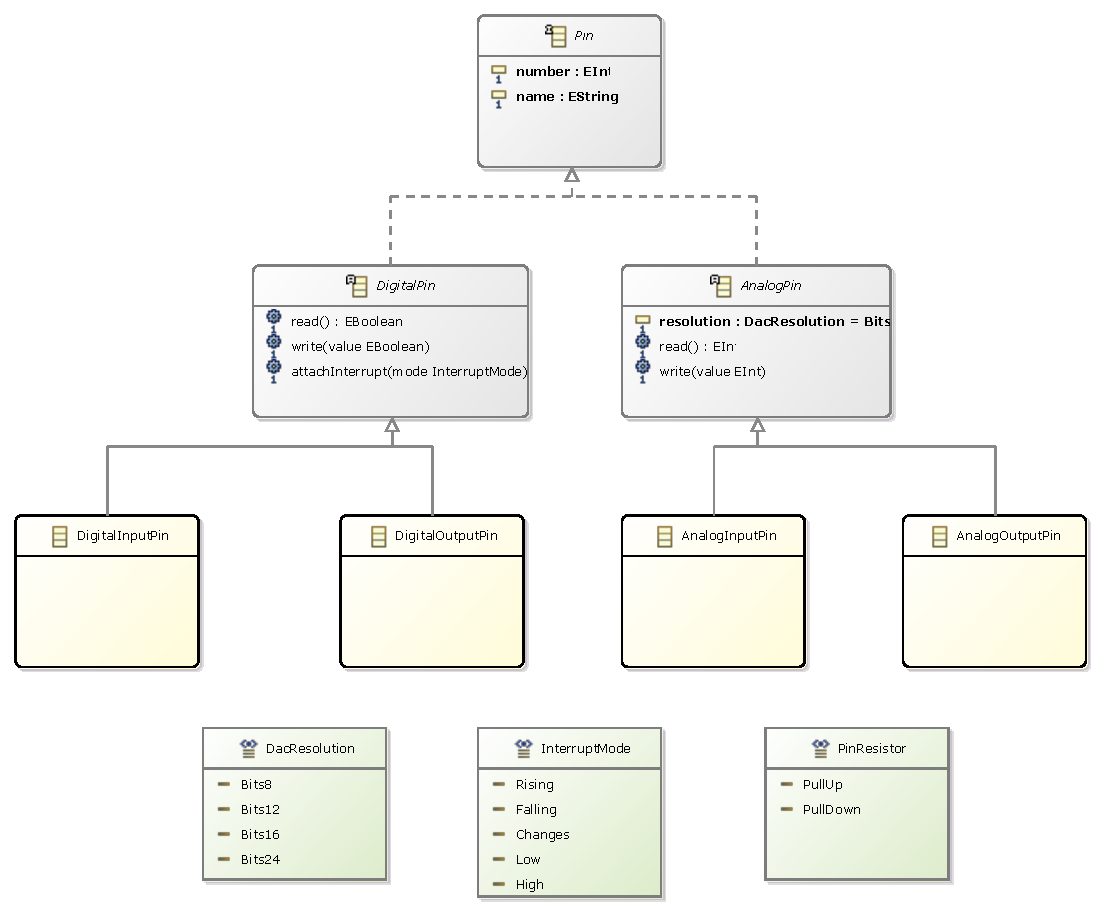
\includegraphics[height=0.3\textheight]{images/models/gpios_class_diagram.pdf}
    \captionmodeloclase{GPIO}
    \label{fig:modelo_iot_gpio_classes}
\end{figure}

\begin{figure}
	\centering
    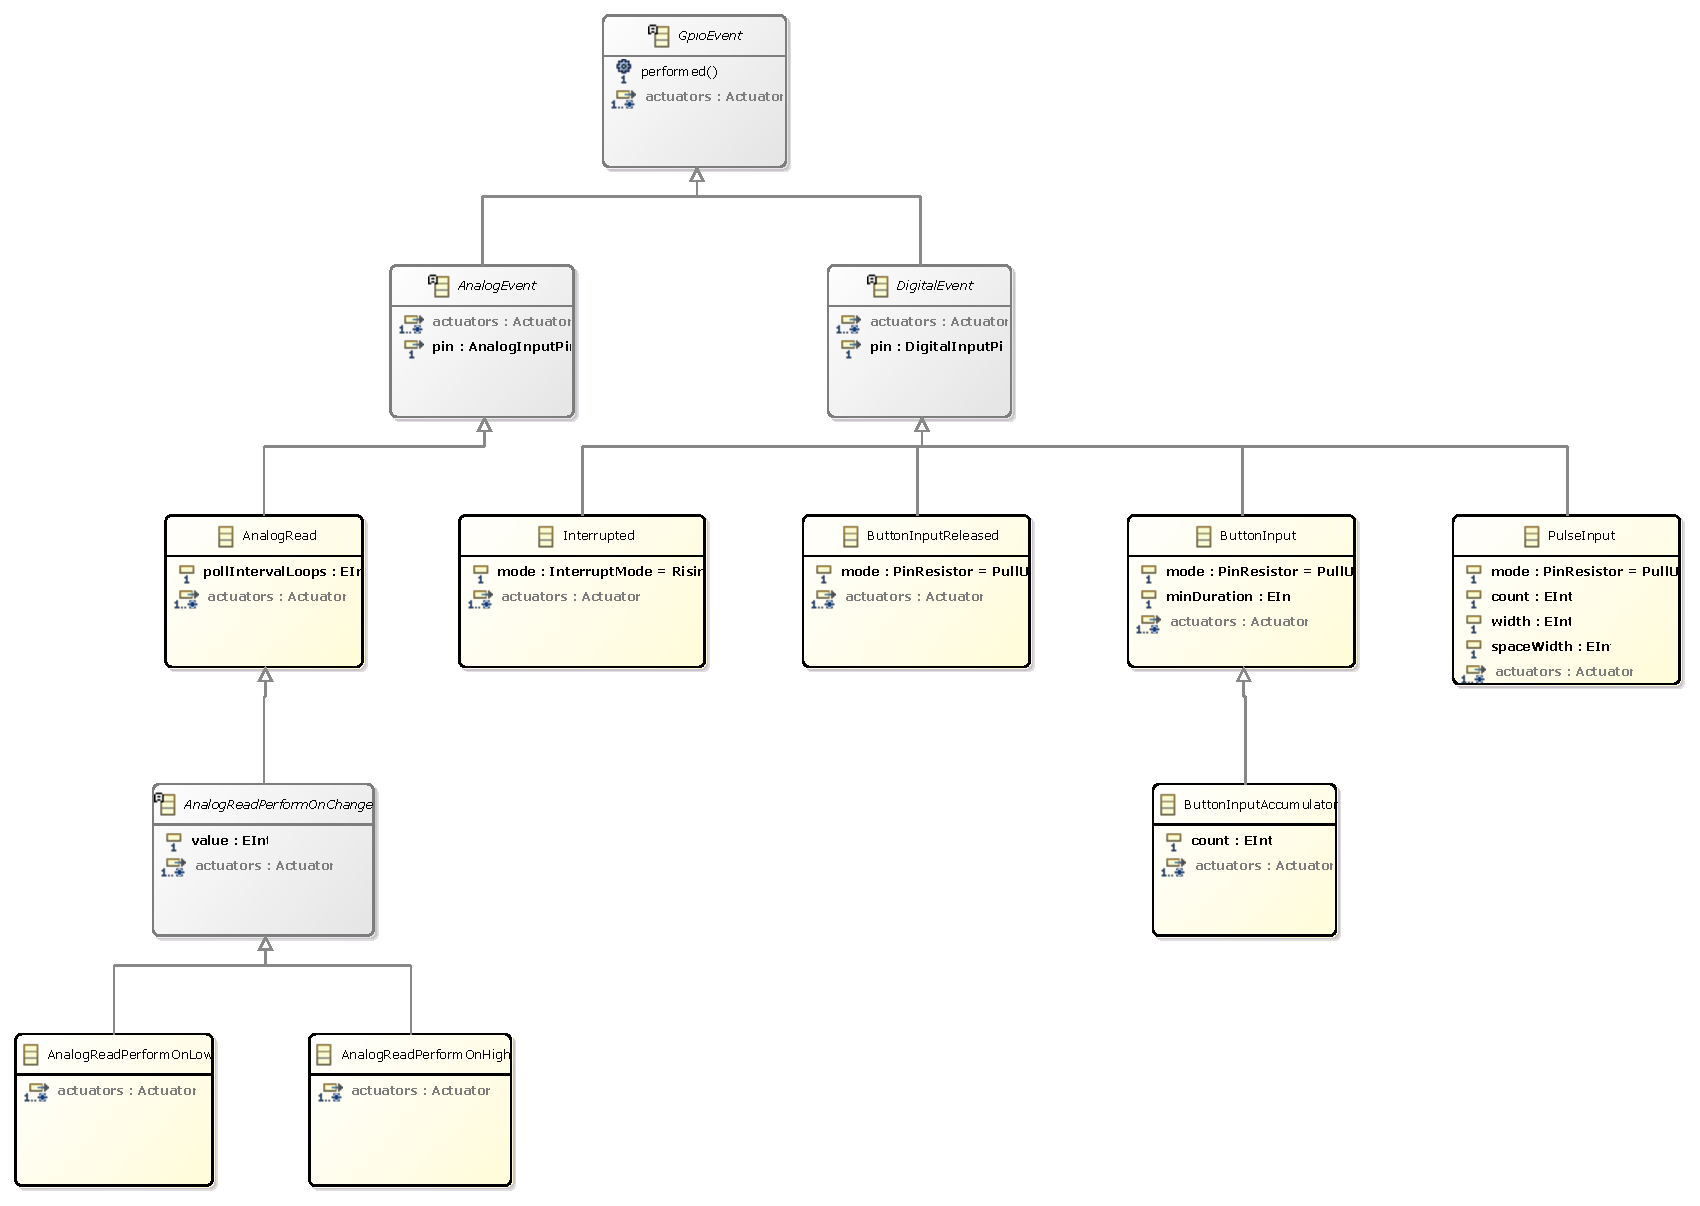
\includegraphics[height=0.3\textheight]{images/models/gpiosevents_class_diagram.pdf}
    \captionmodeloclase{GPIO - Eventos}
    \label{fig:modelo_iot_gpio_events_classes}
\end{figure}

\begin{figure}
	\centering
    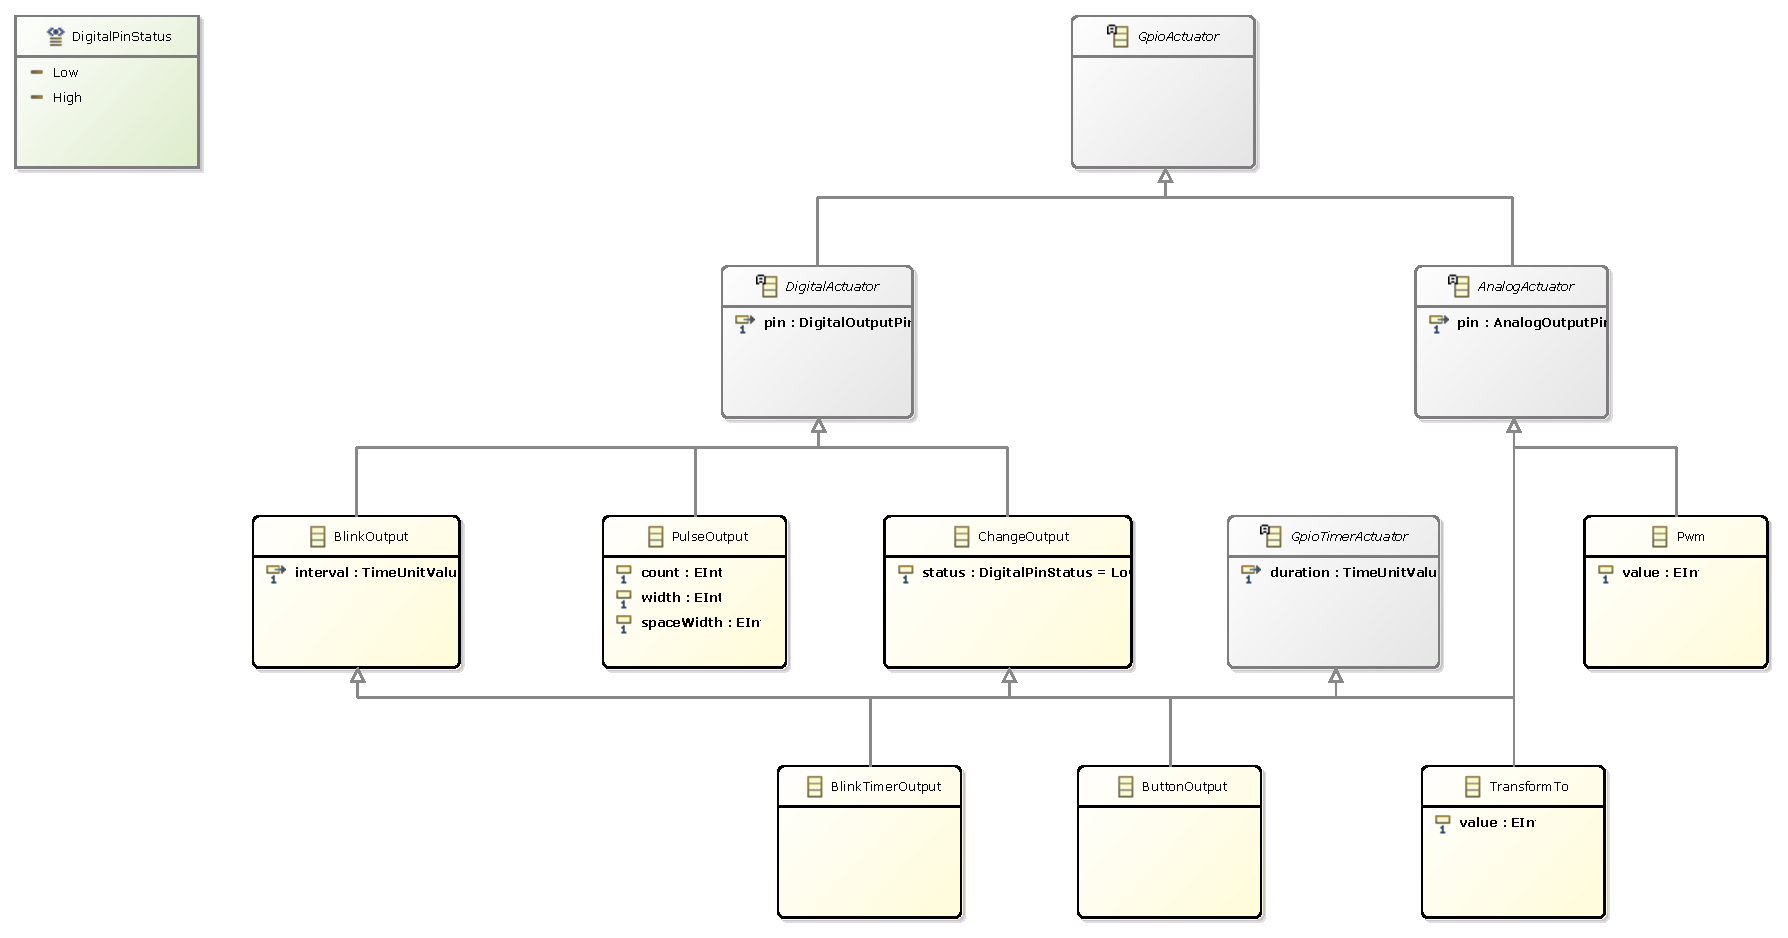
\includegraphics[height=0.3\textheight]{images/models/gpiosactuators_class_diagram.pdf}
    \captionmodeloclase{GPIO - Actuadores}
    \label{fig:modelo_iot_gpio_actuators_classes}
\end{figure}


\subsection{Modelo estado de salud}
\label{modelo_health}

Representa el estado de salud de un dispositivo. La monitorización del estado de salud es una parte esencial del sistema ya que nos permitirá detectar comportamientos anómalos tales como una alta carga en CPU por un fallo seguramente en la programación, una carga anormal de memoria RAM, o detectar una temperatura de procesador demasiada alta para su correcto funcionamiento.
En la siguiente figura \ref{fig:modelo_iot_health_ecore} visualizamos el modelado en formato \gls{ecore} tree. En la figura anexa \ref{fig:modelo_iot_health_classes} podemos ver el modelo de clases.

\begin{figure}
	\centering
    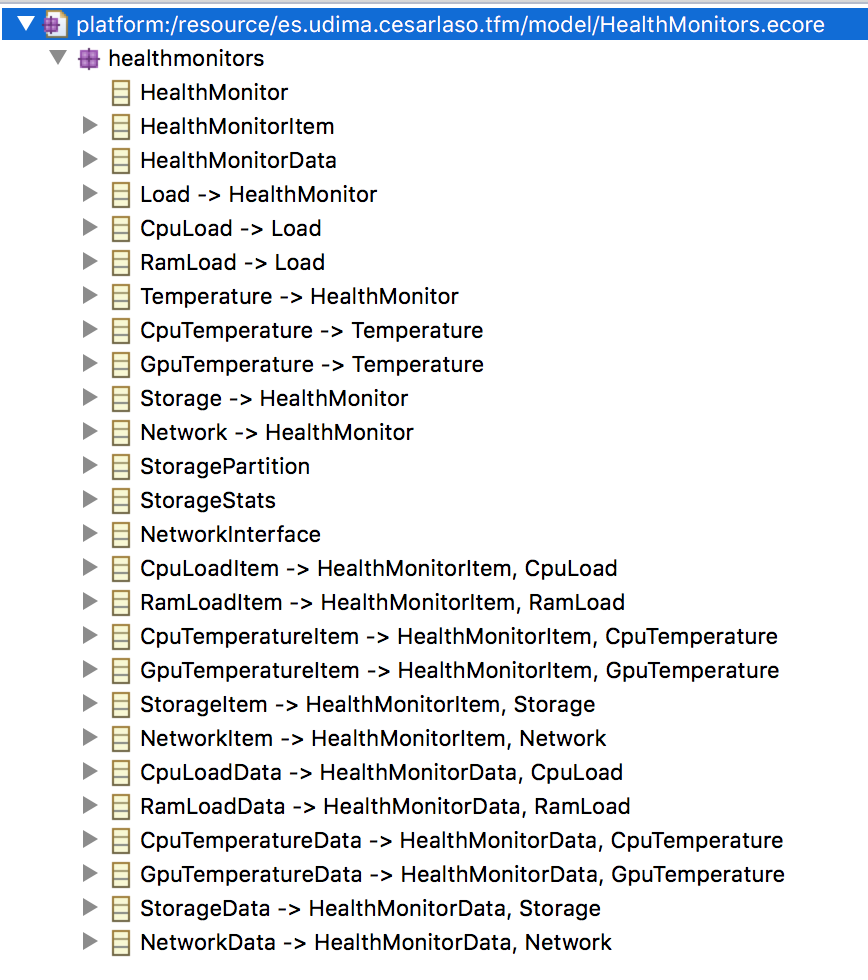
\includegraphics[scale=0.5]{images/emf_capturas/health_ecore.png}
    \captionmodelotree{Health}
    \label{fig:modelo_iot_health_ecore}
\end{figure}

Esta monitorización estará disponible en aquellos dispositivos que funcionen mediante un sistema operativo completo como Linux. Por este motivo, la comprobación del estado de salud no podrá ser aplicada a los dispositivos de tipo microcontrolador ya que al carecer de un sistema operativo completo, correr directamente en el hardware, o correr en un sistema operativo de tiempo real muy limitado no es posible en esta fase actual del desarrollo realizar esta implementación. En líneas futuras podríamos implementar dicha funcionalidad en el sistema operativo FreeRTOS \cite{freertos}, sistema operativo el cual corre el dispositivo ESP8266 \cite{esp8266}.

Este modelo será utilizado por el modelo de comunicación en la sección \ref{modelo_communication_health_services}.

\subsection{Modelos relativos al protocolo de comunicación}

\subsubsection{Modelo: Servicios de comunicación base}

El modelo servicios de comunicación, representa las bases del protocolo de comunicación entre dispositivos \gls{iot} y una serie de servidores centrales o distribuidos.

Como puede observarse en la figura \ref{fig:modelo_servicios_comunicacion_classes}, tenemos la clase principal \textit{Packet}, que contiene los elementos base del protocolo de comunicación: número de secuencia, \gls{timestamp}, servicios.

Un paquete contiene dentro de su \gls{payload} uno o varios servicios, definidos posteriormente en los posteriores modelos.

Este diseño se ha realizado de esta forma ya que puede ser habitual que un dispositivo no tenga conexión con el servidor de forma continua, teniendo este que guardar toda la comunicación en su memoria a largo plazo para posteriormente cuando consigue conexión, reenviar toda esta información.
Al poder utilizar un solo paquete, simplificamos la comunicación al poder reenviar toda esta comunicación en un solo paso.
Igualmente reducimos la sobrecarga en el protocolo subyacente \gls{tcp}, acumulando varios servicios de información en un solo paquete.

También hemos definido los conceptos petición \textit{ServiceRequest}, respuesta a una petición \textit{ServiceResponse} y notificación sin respuesta previa \textit{ServiceNotification} que se utilizarán en otros modelos de comunicación.

A continuación mostramos en la figura \ref{fig:modelo_servicios_comunicacion_classes}, como se visualiza este modelo en otro tipo de visualización en este caso una vista del diagrama de clases generado, con sus tipos de datos y junto a su documentación, todo ello partiendo siempre del mismo modelo \gls{ecore}. 

\begin{figure}
	\centering
    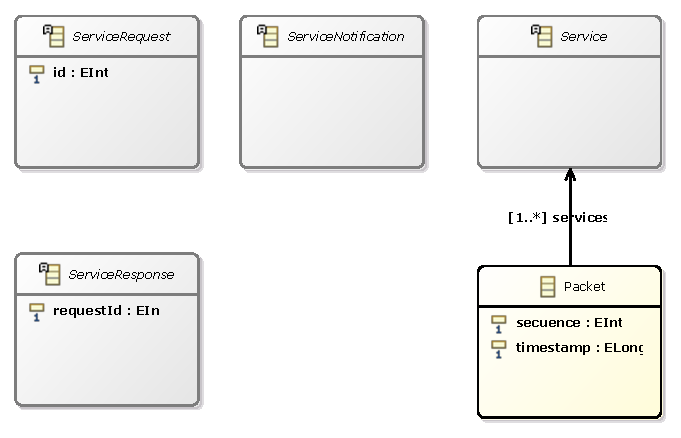
\includegraphics[height=0.3\textheight]{images/models/communications_class_diagram.pdf}
    \captionmodeloclase{Servicios de comunicación}
    \label{fig:modelo_servicios_comunicacion_classes}
\end{figure}

\subsubsection{Modelo: Servicios de comunicación de estado}

El sistema de comunicación necesita mantener la conexión \gls{tcp} para poder tener control del dispositivo desde servidor.
La mayoría de protocolos resuelven este problema enviando un paquete de información de estado cada cierto tiempo si el sistema detecta que no se está enviando información.
El protocolo de nivel inferior utilizado, en el caso propio de este protocolo siendo \gls{tcp}, incluye en su capa de control un modelo de establecer \gls{keepalive}, este sistema cuenta con el problema de su poca configuración en determinados dispositivos y cuenta con un tiempo entre paquetes relativamente alto, del orden de dos horas por defecto en el kernel estandar de Linux. Algunas implementaciones, permiten configurar este parámetro no siendo una configuración sencilla de aplicar a nivel de aplicación. Por este motivo es necesario crear un servicio de control de estado.

Como puede observarse en la figura \ref{fig:modelo_servicios_comunicacion_estado_classes}, contamos con la clase \textit{StatusService} que a su vez implementa la clase del modelo anterior \textit{Service}. A su vez, vemos las clases \textit{Ping} y \textit{Pong} que implementan la clase \textit{StatusService}.

El funcionamiento de este modelo es relativamente sencillo. Si el sistema no detecta actividad en ninguna de las dos direcciones de comunicación, tanto de cliente a servidor como de servidor a cliente en un tiempo determinado, enviará un paquete \textit{Ping}, respondiendo a su llegada el destinatario con un paquete \textit{Pong}.

\begin{figure}
	\centering
    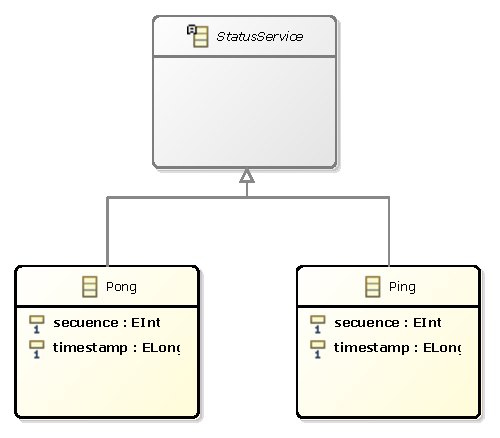
\includegraphics[height=0.3\textheight]{images/models/communicationstatus_class_diagram.pdf}
    \captionmodeloclase{Servicios de comunicación - Estado de conexión.}
    \label{fig:modelo_servicios_comunicacion_estado_classes}
\end{figure}

\clearpage

\subsubsection{Modelo communication health services}
\label{modelo_communication_health_services}

Un sistema \gls{iot} necesita de un buen sistema de monitorización y comunicación de su estado actual de salud, comúnmente llamado \gls{housekeeping}. Podemos evitar posibles problemas en el dispositivo si contamos con la información necesaria.

Para ello, utilizaremos una monitorización constante de variables del sistema tales como cargas de CPU, memoria, tráfico de red, estado de las particiones de disco.
Modelamos el sistema utilizando el modelo \textit{HealthMonitor} el cual define una entidad abstracta de monitorización de salud.

\begin{figure}[ht]
	\centering
    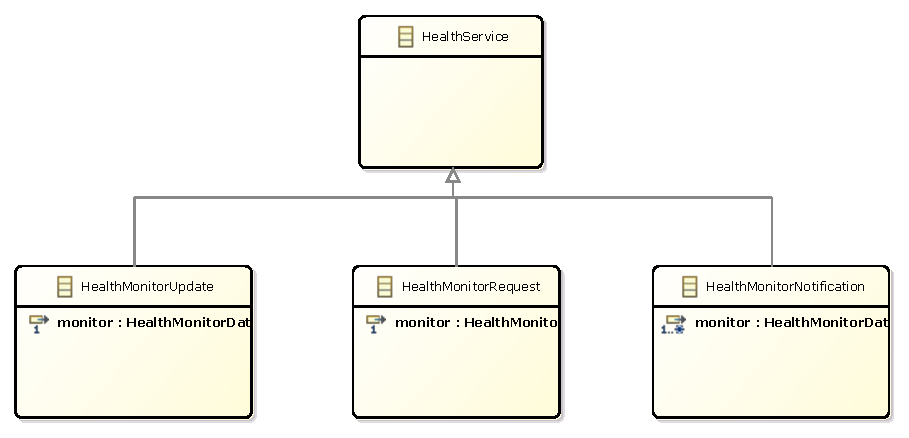
\includegraphics[height=0.3\textheight]{images/models/communicationshealths_class_diagram.pdf}
    \captionmodeloclase{Servicios comunicación - Housekeeping (Estado de salud).}
    \label{fig:modelo_servicios_comunicacion_health_classes}
\end{figure}

Para la comunicación del estado de salud definimos el servicio \textit{HealthService} y dos subservicios tal como puede verse en la figura \ref{fig:modelo_servicios_comunicacion_health_classes}: \textit{MonitorItems} y \textit{MonitorChangeItemInterval}, primer servicio utilizado para enviar el estado de todos los sensores activos desde el dispositivo \gls{iot} al servidor.

El segundo subservicio lo utilizaremos para modificar el intervalo de captura del estado de salud de un elemento en concreto, pudiendo especificar si se desea recuperar la información actual sin esperar al intervalo de tiempo del elemento a monitorizar.

Este modelo necesita de los datos proporcionados el modelo salud en la sección \ref{modelo_health}.

%\subsubsection{Modelo communication events services}

\begin{figure}[ht]
	\centering
    \includegraphics[height=0.3\textheight]{images/models/communication_remote_events_ecore.png}
	\captionmodelotree{Servicios de comunicación - Eventos}
\end{figure}

\begin{figure}[ht]
	\centering
    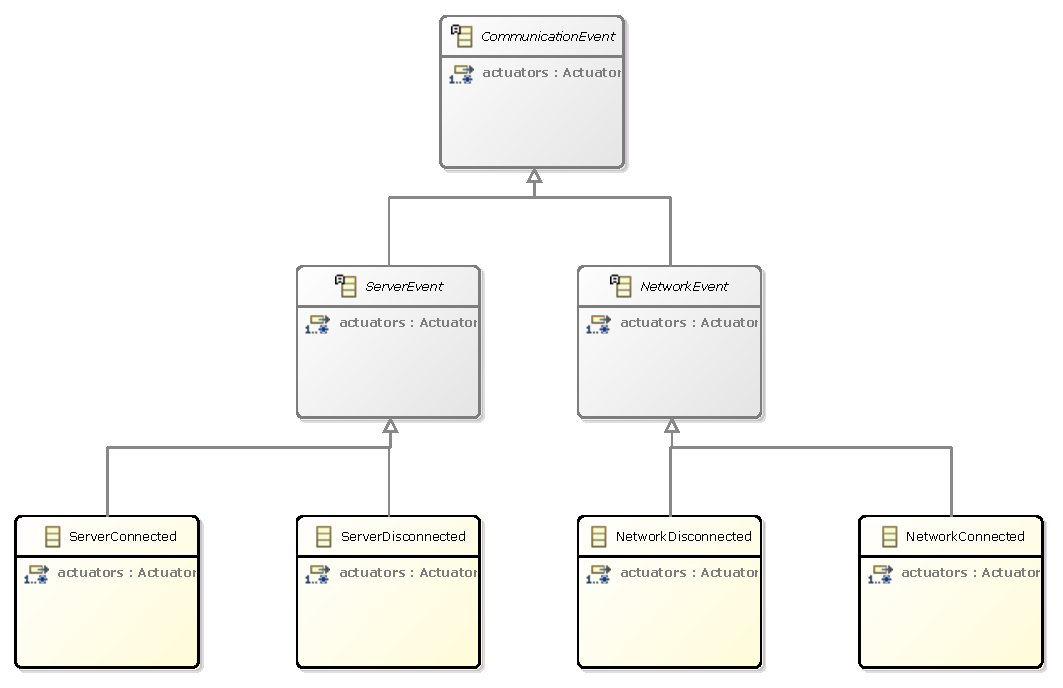
\includegraphics[height=0.3\textheight]{images/models/communicationsevents_class_diagram.pdf}
    \captionmodeloclase{Servicios de comunicación - Eventos}
\end{figure}

\clearpage


\subsubsection{Modelo: Dispositivos}

El modelo Dispositivos presenta las diferentes opciones que tenemos para el despliegue de la aplicación generada por el \gls{dsl} en nuestro dispositivo final.

Como puede observarse en la figura \ref{fig:modelo_dispositivos_classes}, contamos con una serie de dispositivos base, los que tienen sistema operativo completo y la versión Arduino. Todos ellos, comparten el mismo tipo de configuración en este caso solamente tenemos como medio de conexión de red WIFI, compatible con todos los despliegues.

\begin{figure}
	\centering
    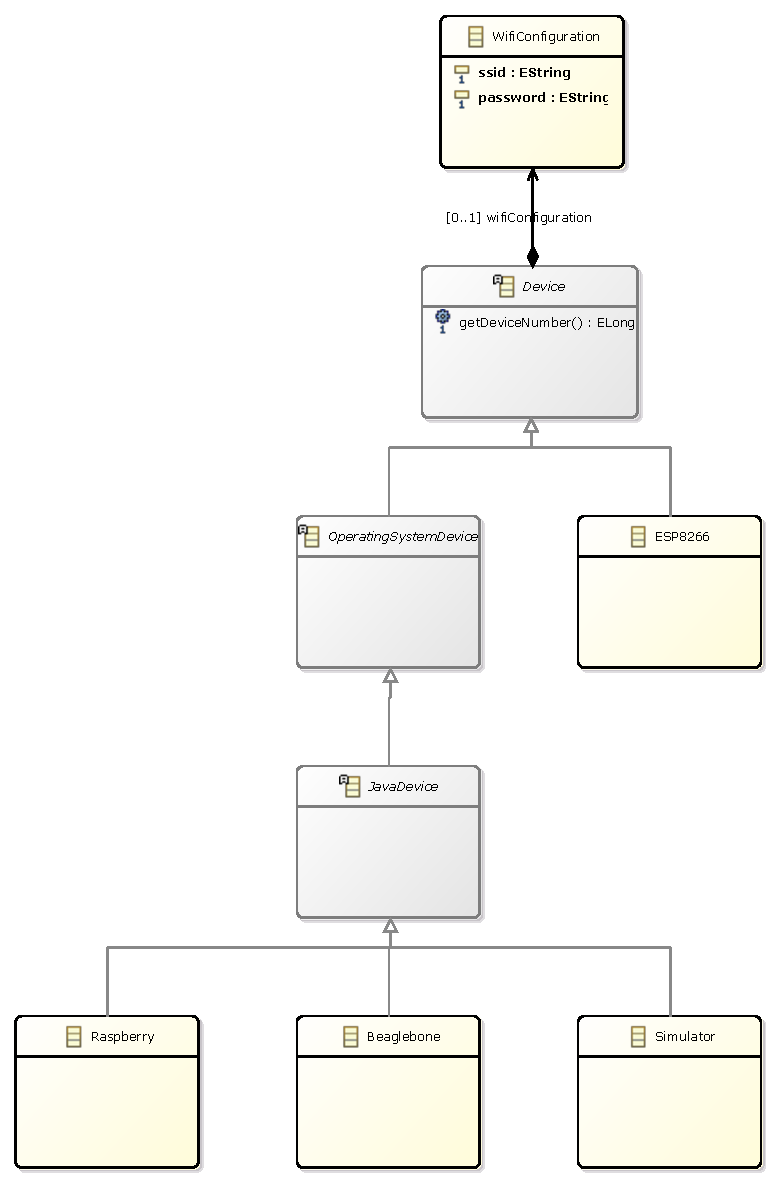
\includegraphics[width=0.4\textheight]{images/models/deploymentdevices_class_diagram.pdf}
    \captionmodeloclase{Dispositivos}
    \label{fig:modelo_dispositivos_classes}
\end{figure}

\subsection{Modelos relativos al servidor y usuarios}

El modelo servidor define un servidor base en el que poder recibir y gestionar los eventos generadores por nuestros dispositivos \gls{iot}. En el modelo, se crea un modelo básico \textit{JavaServer}, el cual es la mínima implementación requerida. La figura \ref{fig:modelo_iot_servidor_classes} muestra un diagrama de clases. 

\begin{figure}
	\centering
    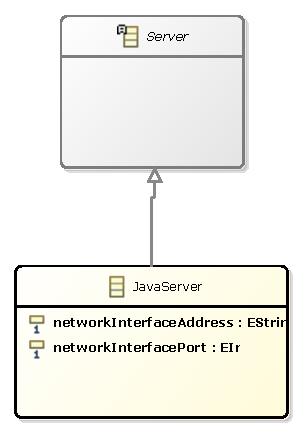
\includegraphics[height=0.3\textheight]{images/models/servers_class_diagram.pdf}
    \captionmodeloclase{Servidor}
    \label{fig:modelo_iot_servidor_classes}
\end{figure}

El modelo usuarios, cuenta con las cualidades que suelen tener los objetos tipo usuario, tales como su nombre, a que compañía pertenece, que dispositivos tiene asignados, conocer si tiene acceso a estos en un determinado momento y en que lugar están situados. La figura \ref{fig:modelo_iot_usuarios_classes} muestra un diagrama de clases.

\begin{figure}
	\centering
    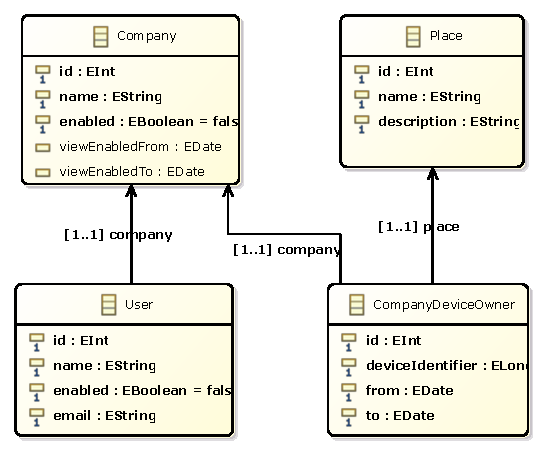
\includegraphics[height=0.3\textheight]{images/models/clients_class_diagram.pdf}
    \captionmodeloclase{Usuarios}
    \label{fig:modelo_iot_usuarios_classes}
\end{figure}

\subsection{Modelos comunes al dominio del dispositivo IOT}

Estos modelos aportan funcionalidades que son transversales a los modelos que componen este proyecto.

\subsubsection{Modelo Eventos/Transacciones}

El modelo eventos representa una transacción base a todos los componentes que posteriormente modelaremos.

%A continuación podemos ver en la figura \ref{fig:modelo_events_ecore} como es representado este modelo. Consiste en dos modelos: \textit{Event} (Evento) , y \textit{Actuator} (Actuador). 

%\begin{figure}[htp]
%	\centering
%    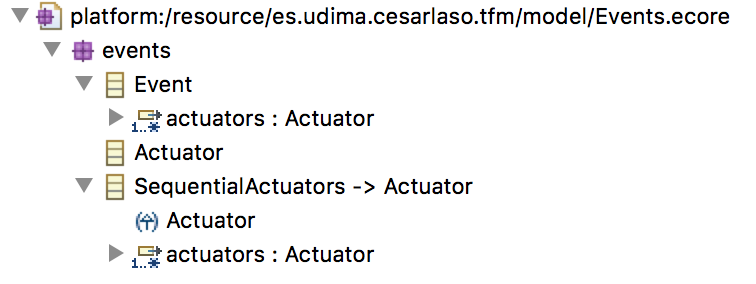
\includegraphics[height=0.3\textheight]{images/emf_capturas/events_ecore.png}
%    \caption{Modelo Events. Visualización formato ecore}
%    \label{fig:modelo_events_ecore}
%\end{figure}



\paragraph{Modelo evento}.
El modelo \textit{Evento} representa una entidad la cual es capaz de generar por sí misma acciones, permite definir los eventos del sistema. Estos pueden ser de diferente naturaleza: aperiódico y periódico.

Como ejemplo de evento aperiódico contamos con un evento de entrada/salida, como puede ser un cambio de estado en una entrada digital. Como ejemplo de evento periódico, contamos con un temporizador el cual es ejecutado cada x unidades de tiempo. 

Un evento siempre contendrá uno o varios actuadores. Un evento sin actuadores no tiene sentido con lo que no está permitido en el modelo.



\paragraph{Modelo actuador}.
El modelo actuador representa una acción a realizar por parte del sistema. Los actuadores dentro del evento se lanzarán de forma concurrente todos al mismo tiempo sin esperar a la finalización de cada uno de ellos. Si fuera necesario mantener un orden en los actuadores, es necesario utilizar el modelo contenedor \textit{SequentialActuactor} el cual en su funcionamiento ejecuta el grupo de actuadores secuencialmente uno tras otro, esperando a la finalización de un actuador para invocar al siguiente.

A continuación en la figura \ref{fig:modelo_events_classes} podemos visualizar esta representación mediante un diagrama de clases.

\begin{figure}[htp]
	\centering
    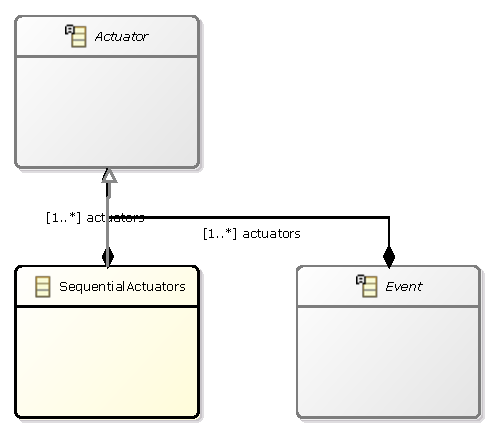
\includegraphics[height=0.3\textheight]{images/models/events_class_diagram.pdf}
    \captionmodeloclase{Eventos / Transacciones}
    \label{fig:modelo_events_classes}
\end{figure}

%\clearpage

\subsubsection{Modelo Timers}

Este modelo representa la funcionalidad de un sistema de eventos por tiempo, ya sea mediante temporizadores periódicos a intervalos concretos o mediante periodos concretos \cite{scheduling_sporadic_aperiodic_events}.

Contamos con los siguientes eventos de tipo:

\begin{itemize}

\item \textit{NowEvent}. Representa un evento para disparar en el mismo momento de su ejecución.
\item \textit{RepeatedEvent}. Representa un evento que disparará cada x unidades de tiempo.
\item \textit{ClockEvent}. Representa un evento que dispará cada x hora/minuto/segundo definidas.
\item \textit{CronEvent}. Representa un evento que dispará cada x unidades definidas en formato Unix CRON.

\end{itemize}

Estos eventos utilizan como tipo de dato los elementos definidos en \textit{TimeUnit} y \texit{TimeUnitValue} para así poder identificar sin ningún error la unidad de tiempo definida.

A continuación podemos visualizar la representación en formato \gls{ecore} en la figura \ref{fig:modelo_timers_ecore} y la representación como diagrama de clases en la figura anexa  \ref{fig:modelo_timers_classes} de este modelo de datos.


El modelo eventos representa la base de todos los componentes que posteriormente modelaremos. Podemos observar en la figura \ref{fig:modelo_timers_ecore} la representación de este modelo en formato \gls{ecore} tree, generado en el propio entorno \gls{emf}.

\begin{figure}
	\centering
    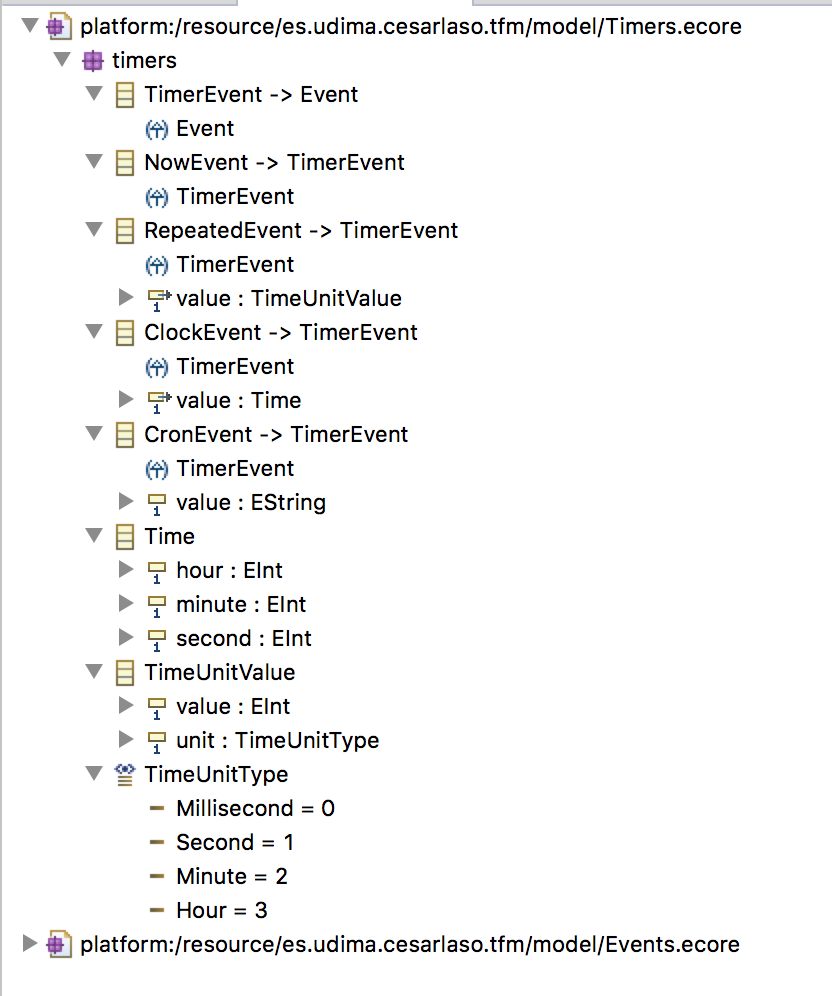
\includegraphics[scale=0.5]{images/emf_capturas/timers_ecore.png}
    \sourcepropia{}
    \captionmodelotree{Timers}
    \label{fig:modelo_timers_ecore}
\end{figure}



\subsubsection{Modelo Proyecto IOT}

\begin{figure}[htp]
	\centering
    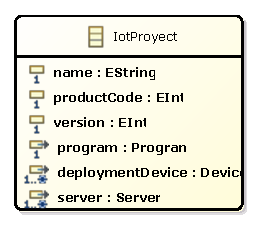
\includegraphics[height=0.2\textheight]{images/models/iotproyects_class_diagram.pdf}
    \captionmodeloclase{Proyecto IOT}
    \label{fig:modelo_iotproyects_classes}
\end{figure}

En el anexo \ref{appendix:modelos_ecore_tree}, podemos observar en la figura \ref{fig:modelo_iotpackages} mostramos el árbol de dependencias entre los diferentes modelos tratados en este proyecto.

\subsubsection{Modelo Programa}

Este modelo conforma la base del programa que posteriormente definiremos en el \gls{dsl}. Es la base del proyecto, a partir de este \gls{metamodelo}, generaremos programas mediante un \gls{dsl} creado con \gls{xtext}. 

Este modelo representa un programa \gls{iot} en el que tenemos una serie de entradas, ya sean desde el propio \gls{gpio}, una serie de entradas remotas y acciones tanto en el propio \gls{gpio} como notificaciones remotas.

Como ejemplo, imaginemos un dispositivo \gls{iot} de lo más simple, con una sola entrada digital, utilizado para contabilizar monedas de una máquina de refrescos. Mediante el \gls{dsl} que definimos en este proyecto podríamos generar un programa para una plataforma determinada que cumpla con las siguientes características: Gestión de la interrupción \gls{gpio} asociada a dicho evento de pulso de entrada de moneda, notificación a servidor de este evento,  control de salud del propio dispositivo, etc.

El programa define una serie de \gls{gpio} pin, indicando estos con un alias, es decir, podemos asignar un nombre a una entrada, por ejemplo, \gls{led} rojo \textrightarrow pin1. Cuenta con asignación de nombres de eventos remotos, y rutas de archivos a utilizar por el programa. Un programa cuenta con una serie de estados, necesario indicar el estado principal de arranque de este y posibilitando cambiar de estado. Un ejemplo de uso real es el testeo en el arranque de los diversos indicadores \gls{led} u otras entradas/salidas, y una vez terminado, pasar a un estado de error en caso de fallo, y en caso de funcionamiento normal, pasar al estado del programa principal.


En la figura \ref{fig:modelo_iot_programa_classes} podemos visualizar en formato diagrama de clases \gls{uml} el modelo \textit{Program}.

\begin{figure}
	\centering
    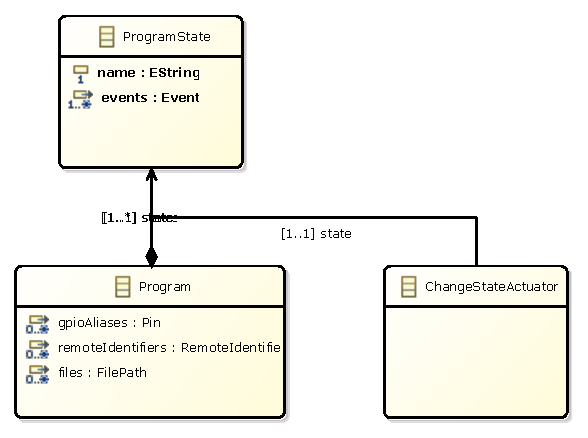
\includegraphics[height=0.3\textheight]{images/models/programs_class_diagram.pdf}
    \captionmodeloclase{Programa IOT}
    \label{fig:modelo_iot_programa_classes}
\end{figure}

\clearpage

